% EAJ - svg generation needs to be run with -shell-escape:
% pdflatex -shell-escape filename.tex
\documentclass[border=2pt, tikz, convert={command=\unexpanded{{pdf2svg \infile\space "\jobname.svg" && rsvg-convert --zoom 1.85 --format svg --output "\jobname.svg" "\jobname.svg" && convert -density 300 \infile\space "\jobname.png"}}}]{standalone}
\begin{document}
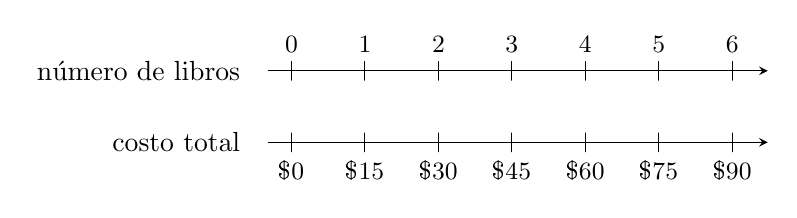
\begin{tikzpicture}

\usetikzlibrary{fit}

%  TikZ Styles for Number Lines
\tikzset{
  tickLabelAbove/.style={
      font=\small,        % Font size for tick labels
      anchor=mid,         % Baseline align text vertically across nodes
      yshift=2.0ex,       % Vertical offset for labels above the line
  },
  tickLabelBelow/.style={
      font=\small,        % Font size for tick labels
      anchor=mid,         % Baseline align text vertically across nodes
      yshift=-2.6ex,      % Slightly larger offset below the line to account 
                          % for the label's baseline alignment (ensures visual balance).
  },
  numLineTick/.style={
      draw,               % Draw tickmark node
      minimum width=0pt,  % No width for the node box
      minimum height=7pt, % Height of the tickmark
      line cap=round,     % Rounded ends for ticks
      inner sep=0pt,      % No inner padding
      outer sep=2pt,      % Space around the tick
      line width=0.35pt,  % Thickness of the tick line
  },
}

\newcommand{\doubleNumberLine}[6]{%
  % Parameters:
  % #1: Number line lengths (without the label)
  % #2: Number of marks
  % #3: Top mark labels (comma-separated)
  % #4: Top line label (placed at the left)
  % #5: Bottom mark labels (comma-separated)
  % #6: Bottom line label (placed at the left)

   % Internal constants
  \def\numLineExtra{0.3cm} % Hardcoded extra space at the ends
  
  %%% TOP number line
  \begin{scope}
    % Coordinates of endpoints
    \coordinate (top-leftEnd) at (0, 0);
    \coordinate (top-rightEnd) at (#1, 0);

    % Draw the number line and add label to the left
    \draw[->, >=stealth] (top-leftEnd) -- (top-rightEnd);
    \node[anchor=east, xshift=-1.5ex] at (top-leftEnd) {#4};

    % draw ticks as nodes (top-mark-n). 1st mark is (top-mark-1).
    \foreach \x in {1,...,#2}{%
        \node[numLineTick] (top-mark-\x) at ({\numLineExtra+(\x-1)*(#1-2.5*\numLineExtra)/(\numMarks-1)},0) {};
    }

    % add mark labels
    \foreach \num [count=\i] in #3 {
        \node[tickLabelAbove] at (top-mark-\i) {\num};
    }
  \end{scope}

  %%% Bottom number line
  \begin{scope}[yshift=-6ex]
    % Coordinates of endpoints
    \coordinate (bot-leftEnd) at (0, 0);
    \coordinate (bot-rightEnd) at (#1, 0);

    % Draw the number line and add label to the left
    \draw[->, >=stealth] (bot-leftEnd) -- (bot-rightEnd);
    \node[anchor=east, xshift=-1.5ex] at (bot-leftEnd) {#6};

    % draw ticks as nodes (bot-mark-n). 1st mark is (bot-mark-1).
    \foreach \x in {1,...,#2}{%
        \node[numLineTick] (bot-mark-\x) at ({\numLineExtra+(\x-1)*(#1-2.5*\numLineExtra)/(\numMarks-1)},0) {};
    }

    % add mark labels
    \foreach \num [count=\i] in #5 {
        \node[tickLabelBelow] at (bot-mark-\i) {\num};
    }
  \end{scope}
}

% Parameters
\def\lineWide{2.5in} % width of line (not including label)
\def\numMarks{7}
\def\topMarkLabels{0,1,...,6} 
\def\topLineLabel{número de libros}
\def\bottomMarkLabels{\$0, \$15, \$30, \$45, \$60, \$75, \$90} 
\def\bottomLineLabel{costo total}

% Draw double number line
% creates several coordinates like (top-leftEnd) and (bot-mark-2). See details in template.
\doubleNumberLine{\lineWide}{\numMarks}{\topMarkLabels}{\topLineLabel}{\bottomMarkLabels}{\bottomLineLabel}

% Extra text in marks if needed
% \node[tickLabelBelow] at (top-mark-3) {text below};

% box around some top and bottom marks
% \node[fit=(top-mark-4) (bot-mark-4), draw, rectangle, rounded corners=1.5ex, inner sep=2.7ex, densely dashed] {};

\end{tikzpicture}
\end{document}